\documentclass{article}

% ---------------------------------------------------------------------------
% Preamble: uses the official NeurIPS 2026 style if present, otherwise a
% self-contained fallback so the file compiles standalone.
% ---------------------------------------------------------------------------
\PassOptionsToPackage{numbers,compress}{natbib}
\IfFileExists{neurips_2026.sty}{%
  \usepackage[preprint]{neurips_2026}%
}{%
  \usepackage[margin=1in]{geometry}%
  \usepackage{times}%
  \usepackage[T1]{fontenc}%
  \newcommand{\And}{\quad}%
}
\makeatletter
\@ifpackageloaded{natbib}{}{\usepackage[numbers,compress]{natbib}}
\makeatother

\usepackage{graphicx}
\usepackage{booktabs}
\usepackage{amsmath}
\usepackage{xcolor}
\usepackage{microtype}
\usepackage{url}
\usepackage[colorlinks=true,linkcolor=blue,citecolor=blue,urlcolor=blue]{hyperref}

\emergencystretch=1.5em

% Red bracketed marker for results that land in the camera-ready.
\newcommand{\pending}[1]{{\color{red}[\textsc{pending}: #1]}}
\newcommand{\todo}[1]{{\color{red}[TODO: #1]}}

\title{Beyond File Overlap: Semantic Conflicts Between Concurrent AI Coding Agent Pull Requests}

% ---------------------------------------------------------------------------
% ANONYMIZED SUBMISSION. Restore the camera-ready author block only after
% checking the workshop's anonymity policy.
% ---------------------------------------------------------------------------
\author{Anonymous Author(s)}
\date{}

\begin{document}
\maketitle

\begin{abstract}
Autonomous coding agents now open pull requests (PRs) concurrently in the same repositories, and the interference signal used to verify their concurrent work today---by orchestrators, measurement studies, and benchmarks alike---is textual: do two changes touch the same file? Analyzing 577{,}045 co-active agent PR pairs from the AIDev corpus, we show that this signal errs in both directions. % src: verification_log.md sizes/anatomy (577,045 pairs)
Among the 42{,}600 pairs (7.38\%, 95\% CI [7.32, 7.45]) that share a changed file, 33.9\% share \emph{only} manifests, lockfiles, CI configuration, or documentation, and 65.0\% share exactly one file. % src: p1_headline_cis.json (conflict_rate_all_pairs, pure_config, share_exactly_one_file)
Conversely, deterministic candidate pools expose interference that file overlap cannot see: 79.6\% of 6{,}945 near-duplicate-title pairs share no file at all, and 46.8\% of the pool merged \emph{both} PRs---candidate redundant work landing twice, half of it within the hour. % src: p1_headline_cis.json dup_no_shared_file, dup_both_merged; dup_detail.json
We contribute (i) a taxonomy of semantic conflict between concurrent agent PRs (duplicate work, contradictory changes, dependency-mediated interference, harmful vs.\ benign co-editing) grounded in classic software-merging definitions; (ii) the first in-the-wild, corpus-scale measurement of semantic-conflict candidates between concurrent agents' PRs, with exact pool definitions and Wilson intervals; (iii) the first pair-level analysis linking these categories to PR fate \emph{for concurrent agent PRs}, via repo-stratified Mantel--Haenszel odds ratios that reverse two crude associations (duplicate-title pairs' later PRs merge \emph{more} often within-repo, OR 1.51 [1.39, 1.63]); % src: p1_outcomes.json b_dup_title_vs_rest
(iv) an exhaustive case study of all 99 cross-agent candidate pairs across the three enumerable pools; and (v) a pre-specified LLM-judge and human-validation pipeline with its 8{,}949-pair judging frame, inclusion probabilities, and calibration sheet released; pool statistics are candidate counts, and the judge run over that released frame is the named computation that bounds their precision. File-level conflict checking, the de facto verification signal for concurrent agent work, is measurably wrong in both directions---the artifact that needs verification is the \emph{pair}.
\end{abstract}

\section{Introduction}
\label{sec:intro}

Autonomous coding agents ship work as pull requests, and they increasingly do so \emph{concurrently}: in the curated AIDev-pop corpus of 33{,}596 agent PRs across 2{,}807 repositories \citep{li2026aidev,li2025rise}, prior work established that 79.4\% of agent PRs are co-active with at least one other agent PR in the same repository, forming 580{,}913 co-active pairs, and that replaying a stratified sample of 747 such pairs with three-way merges yields textual conflict rates of 19.8\% intra-agent and 41.7\% cross-agent \citep{xu2026agentprs}. % src: arXiv:2607.04697 (cited)
A parallel effort measured a 27.67\% PR-vs-mainline textual conflict rate among the ${\sim}107$K agent PRs (of 142{,}652 collected) that completed deterministic merge simulation \citep{agenticflict}. % src: [agenticflict] (cited); verification_log.md external
Both studies rest on the same verification primitive---a conflict exists iff two changes collide \emph{textually}---and many practical orchestration pipelines gate on the same file-level signal. Both studies explicitly disclaim semantic or logical conflicts as unmeasured future work, while practitioners assert that exactly this implicit, semantic interference between parallel agents is the binding reliability constraint \citep{cognition2025,coagent}.

File overlap is neither necessary nor sufficient for real interference. Two anecdotes from the corpus studied here: in \texttt{Cap-go/capgo}, PRs \#1091--\#1093 and \#1095 fix the same bug repeatedly---three TypeScript trigger edits and one SQL migration---with the TS-vs-SQL pairs sharing \emph{zero} files, so every file-level check reports ``no conflict''; % src: design doc / manual inspection of predictor false positives
in \texttt{wix/react-native-ui-lib}, PR \#3631 (``Revert formatting changes in multiple components'') explicitly undoes agent PR \#3626---one agent unwinding another's landed work. % src: ev_semantic.md contradiction pool (1 pair citing partner PR)
Neither failure mode is visible to the signal the field currently measures, predicts, and schedules against.

This paper measures the gap. We define \emph{semantic conflict} between co-active agent PRs, operationalize it without executing code, and quantify what today's file-level signal gets wrong on all 577{,}045 co-active pairs with file data on both sides. % src: verification_log.md (577,045)
Our claims are deliberately scoped: \citet{xu2026agentprs} and \citet{agenticflict} own textual conflict measurement, \citet{cooperbench} own constructed-and-executed two-agent cooperation benchmarks, and \citet{duppr} own duplicate-PR measurement in human OSS. What no prior study provides---and what we claim---is (a) the \emph{first in-the-wild, corpus-scale measurement of semantic-conflict candidates between concurrent agents' PRs}, and (b) the \emph{first pair-level analysis linking semantic-conflict categories to PR fate for concurrent agent PRs} (\citet{li2022duplicates} did so for human duplicate-PR pairs). We state the corpus composition up front because it shapes every estimate: 92.2\% of pairs are Codex--Codex, and two repositories account for 87.3\% of all pairs, % src: verification_log.md anatomy (92.2451%; 87.2946%)
so we report repo-stratified and mega-repo-excluded numbers throughout, and we speak of ``concurrent agent PRs'' (mostly same-agent fan-out) rather than ``concurrent agents'' except where cross-agent evidence is explicitly enumerated (\S\ref{sec:crossagent}).

\textbf{Contributions.}
\begin{enumerate}
  \item \textbf{Taxonomy} (\S\ref{sec:taxonomy}): four categories of semantic conflict for concurrent agent PRs---\textbf{D}uplicate work, \textbf{C}ontradictory changes, dependency-mediated \textbf{I}nterference, and \textbf{H}armful-vs-\textbf{B}enign co-editing---mapped onto the classic definition families (Horwitz interference, Palant\'ir indirect conflicts, plan invalidation), with I explicitly demoted to a \emph{candidate signal} pending non-textual validation.
  \item \textbf{Both-direction error anatomy of file overlap} (\S\ref{sec:anatomy}): 33.9\% of file-overlap conflicts touch only config/docs; 65.0\% share exactly one file; conversely 79.6\% of near-duplicate-title pairs share no file, and all 7 high-confidence false positives of a zero-shot conflict predictor are duplicate-task siblings in disjoint files. % src: p1_headline_cis.json; verification_log.md prediction #8
  \item \textbf{Candidate-pool volumes and outcome coupling} (\S\ref{sec:pools}--\S\ref{sec:outcomes}): five deterministic candidate pools over all 577k pairs with exact definitions, Wilson CIs, and repo-stratified Mantel--Haenszel merge-odds ratios, including Simpson reversals that flip the sign of two crude associations.
  \item \textbf{Cross-agent case study} (\S\ref{sec:crossagent}): exhaustive enumeration of all 99 cross-agent candidate pairs across three pools.
  \item \textbf{A pre-registered measurement pipeline} (\S\ref{sec:pipeline}): a rubric-guided LLM judge over a capped, stratified frame with human calibration \emph{before} the full run, blind dual-annotator validation, leakage scrubbing, and inverse-inclusion-probability weighting; the frame (8{,}949 pairs), inclusion probabilities, rubric, and calibration sheet are released; judge precision per pool, calibration $\kappa$, and population-weighted prevalence are the remaining named computations over that frame, not claims of this version. %% FILL-IN F: after 05/06, replace with: ``the calibration round reaches $\kappa=$XX and per-pool judge precision is reported in Table~\ref{tab:judged}; population-weighted prevalence follows the 300-pair validation.''
 Pool statistics in this version are candidate volumes, not prevalence estimates.
\end{enumerate}

\section{Background and related work}
\label{sec:related}

\textbf{Classic software merging.} Semantic interference between program variants was formalized by \citet{horwitz1989integrating} via program-dependence graphs; \citet{mens2002survey} established the textual/syntactic/semantic merge taxonomy and that semantic conflict detection is undecidable in general---every scalable detector is a proxy. Palant\'ir \citep{palantir} distinguished \emph{direct} conflicts (same artifact) from \emph{indirect} conflicts (different artifacts interacting through dependencies), detectable statically. Crystal \citep{crystal} showed via speculative merging across nine OSS systems that many conflicts manifest only as build/test failures after a textually clean merge; Cassandra \citep{cassandra} measured textual conflict rates of 7.6--19.3\% of merges and scheduled tasks to avoid them; % src: [cassandra] (cited)
\citet{brindescu2020merge} showed conflict-implicated code is ${\sim}2\times$ as bug-prone. On the detection side, SafeMerge verified semantic conflict freedom on 52 merges, flagging 13 and confirming 11 genuine violations, several invisible to textual merge \citep{safemerge}; % src: [safemerge] (cited); verification_log.md external
SAM detects behavior change with generated tests \citep{sam2024}; and \citet{dejesus2023static} showed execution-free static detection is viable---the methodological precedent we scale. Conflict \emph{prediction} \citep{owhadi2019predicting} and neural conflict \emph{resolution} \citep{mergebert,deepmerge,mergebenchconf,conflictbench} both consume the textual conflict label whose validity we interrogate here.

\textbf{The agent era.} AIDev \citep{li2026aidev,li2025rise} collected 932{,}791 agent PRs and defines the curated 33{,}596-PR/2{,}807-repo subset we analyze (termed AIDev-pop by \citet{xu2026agentprs}). % src: [aidev] (cited)
\citet{xu2026agentprs} measured co-activity and replayed textual conflicts on this corpus; AgenticFlict \citep{agenticflict} measured PR-vs-mainline textual conflicts without pairing. Single-agent benchmarks verify one patch in isolation \citep{swebench,swegym}; CooperBench \citep{cooperbench} constructs 652 two-agent tasks with intentionally embedded conflicts and executes merged tests, reporting a ${\sim}30\%$ success drop under cooperation---constructed and execution-based, where we mine naturally occurring pairs at corpus scale and couple them to real PR outcomes. % src: [cooperbench] (cited)
BulkPR-Bench \citep{bulkprbench} lifts the constructed setting to the set level---agents must identify interactions among 581 queued PRs across 18 repos and deliver the largest safe subset---again a constructed, execution-based queue-governance benchmark, where we measure naturally occurring pairs and their real fates. % src: [bulkprbench] (cited)
Coordination mechanisms are proliferating \citep{caid,coagent,grite,spoq}; notably, grite \citep{grite} does \emph{measure} duplicate-and-conflicting work---reporting large reductions under its own git-native coordination substrate---but instruments its own controlled substrate rather than observing the wild population of GitHub agent PRs. AIDev-based studies of agent-PR \emph{rejection} \citep{rejection2026,ehsani2026fail} analyze single-PR outcomes---the qualitative taxonomy of \citet{ehsani2026fail} already names duplicate agent PRs as a rejection pattern---whereas our outcome analysis is pair-level and corpus-scale. Duplicate work is a decade-old measured phenomenon in human OSS---DupPR manually verified 2{,}323 duplicate PR pairs \citep{duppr}, and \citet{li2022duplicates} linked human duplicate pairs to integrator preference and acceptance at the pair level---and our category D is best read as \emph{DupPR in the agent era}: the new elements are co-activity (simultaneous, not sequential fork duplicates), cross-agent duplication, and the both-merged redundancy outcome. Finally, ``semantic conflict'' is also used for contradictions among agent \emph{messages} in multi-agent LLM systems \citep{semcons2026}; our subject is conflicts between code artifacts.

\section{Defining semantic conflict for concurrent agent PRs}
\label{sec:taxonomy}

A co-active pair $(A,B)$ of agent PRs is \emph{semantically conflicting} if merging both would change the meaning or value of either contribution, regardless of whether they collide textually. We partition this into four categories, each grounded in a classic definition family (Table~\ref{tab:taxonomy}).

\begin{table}[t]
\centering
\caption{Taxonomy of semantic conflict between co-active agent PRs, the classic definition family each category descends from, and its execution-free operationalization. Category I is a \emph{candidate signal}: it cannot be validated from patch excerpts alone, so this paper reports its recall-oriented pool and defers precision claims to the repo-browsing deep-dive of \S\ref{sec:pipeline}.}
\label{tab:taxonomy}
\small
\begin{tabular}{@{}p{0.20\linewidth}p{0.26\linewidth}p{0.20\linewidth}p{0.24\linewidth}@{}}
\toprule
Category & Definition & Classic family & Candidate pool (recall) \\
\midrule
\textbf{D} Duplicate work & Both PRs implement the same task; at most one is needed & Duplicate PRs \citep{duppr}; plan redundancy & Near-duplicate normalized titles \\
\textbf{C} Contradictory changes & One PR undoes or negates the other, incl.\ fixing the partner's still-open work & Plan invalidation \citep{coagent,cognition2025} & Revert-marker titles; fix-in-flight keyword rule \\
\textbf{I} Dependency interference (\emph{candidate}) & Disjoint files, interacting code: changed signature vs.\ use-site, config key vs.\ consumer & Indirect conflicts \citep{palantir}; static interference \citep{dejesus2023static} & No shared file but shared depth-2 directory \\
\textbf{H/B} Harmful vs.\ benign co-editing & Same file, colliding intent (H) vs.\ mechanical co-edits of lockfiles/docs (B) & Direct/textual conflicts \citep{mens2002survey} & File-overlap pairs, split by file-class composition \\
\bottomrule
\end{tabular}
\end{table}

Categories D and C are intent-level (plan/task) conflicts; H/B refines the direct/textual layer that current measurements stop at; I ports Palant\'ir's indirect conflict to agent PRs. Because semantic conflict is undecidable in general \citep{mens2002survey}, every operationalization is a proxy; we choose the two families that need no execution (static-indirect and intent-level) and pair each recall-oriented pool with a precision-oriented judged layer (\S\ref{sec:pipeline}). We demote I throughout: judging ``A breaks B's call-site'' from two patch excerpts cannot establish that the interaction is real, so I appears here only as a pool (depth-2 near-misses) whose judged precision is deferred.

\section{Data, candidate pools, and measurement pipeline}
\label{sec:data}

\subsection{Data}
We use the curated subset of AIDev \citep{li2026aidev} termed AIDev-pop by \citet{xu2026agentprs}: 33{,}596 agent PRs (OpenAI Codex, Devin, GitHub Copilot, Cursor, Claude Code) from 2{,}807 repositories with $>$100 stars. % src: [aidev]/verification_log.md
Our unit is the co-active pair: two agent PRs in the same repo whose open intervals overlap. Of the 580{,}913 co-active pairs reported by \citet{xu2026agentprs} (580{,}908 rows in the released pair table), \textbf{577{,}045} have changed-file lists for both PRs and form our base population (3{,}863 pairs of the released table dropped for missing file data); % src: verification_log.md anatomy pre-check (580,908 - 577,045 = 3,863)
\textbf{42{,}600} (7.38\%, Wilson 95\% CI [7.32, 7.45]) share $\geq$1 changed file. % src: p1_headline_cis.json conflict_rate_all_pairs
Same-agent pairs conflict at 7.30\% ($n=574{,}187$) and cross-agent pairs at 24.42\% [22.88, 26.03] ($n=2{,}858$); Figure~\ref{fig:agentmatrix} breaks both rates down by unordered agent pair. % src: verification_log.md anatomy; p1_headline_cis.json conflict_rate_cross_agent; fig_p1_agentmatrix
By construction \texttt{pr\_b} is the later-opened PR in every pair. The conflict label was independently re-derived from raw file lists with zero disagreements over all 577{,}045 pairs. % src: verification_log.md outcomes-pools note
Two caveats: PR bodies in our text table are hard-truncated at 1{,}200 characters (21.58\% of bodies hit the cap), so all text-based pools below are computed on truncated text; % src: verification_log.md prediction #10
and merge \emph{times} are proxied by close timestamps (all merged PRs have real close timestamps; zero censored timestamps enter any gap analysis because censored PRs are never merged). % src: verification_log.md merge-time caveat

\begin{figure}[t]
\centering
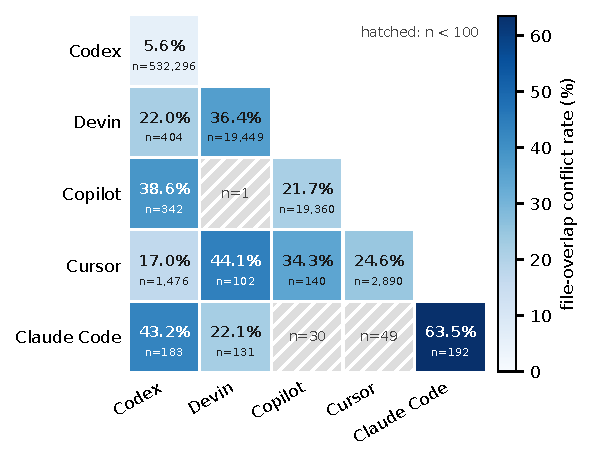
\includegraphics[width=0.52\linewidth]{fig_p1_agentmatrix.pdf}
\caption{File-overlap conflict rate by unordered agent pair over all 577{,}045 co-active pairs. Cells print rate and pair count $n$; color is normalized over cells with $n\geq100$ only; hatched cells ($n<100$) show $n$ only. Diagonal (same-agent): Codex 5.6\% ($n=532{,}296$), Devin 36.4\% ($n=19{,}449$), Copilot 21.7\% ($n=19{,}360$), Cursor 24.6\% ($n=2{,}890$), Claude Code 63.5\% ($n=192$); cross-agent cells with $n\geq100$ span 17.0\% (Cursor--Codex, $n=1{,}476$) to 44.1\% (Cursor--Devin, $n=102$). ``Codex'' denotes OpenAI Codex.} % src: fig_p1_agentmatrix crosscheck (all 15 cells match)
\label{fig:agentmatrix}
\end{figure}

\subsection{Candidate pools (computed on all 577{,}045 pairs)}
\label{sec:pooldefs}

Table~\ref{tab:pools} lists the five deterministic pools. Exact definitions (all reproducible from released code):
\textbf{Duplicate-title}: titles lowercased, \texttt{[...]}-tags deleted, non-alphanumerics to spaces, whitespace collapsed; a pair matches if token-set Jaccard $\geq 0.5$ or one normalized title contains the other with both $\geq$15 characters; both titles must have $\geq$3 tokens. % src: verification_log.md dup pool (caveat 5)
\textbf{Revert-marker}: word-boundary regex \texttt{\textbackslash b(revert|undo|rollback)\textbackslash b} on lowercased titles (plain substring matching would inflate the pool to 342, e.g.\ ``undocumented''). % src: verification_log.md revert pool (caveat 6)
\textbf{Fix-in-flight}: file-overlap pairs whose later PR's normalized title contains a token in \{fix, fixes, fixed, fixing, bug, bugs, bugfix, hotfix, patch, patches, patched\}; keyword-rule variants span 7{,}791--8{,}281 pairs, so we print the exact rule's 7{,}872. % src: verification_log.md fix-in-flight (caveat 7)
\textbf{Depth-2 near-miss}: no shared file, but the two PRs' changed-file directory prefixes (first two path components; repo-root files excluded) intersect. % src: ev_semantic.md §1 depth-2 rule
\textbf{Both-merged + shared file}: file-overlap pairs where both PRs merged; used only descriptively---it conditions on the outcome and is excluded from all odds-ratio analyses (\S\ref{sec:outcomes}).

\begin{table}[t]
\centering
\caption{Deterministic candidate pools over all 577{,}045 co-active pairs. Pools are recall-oriented candidate sets, not confirmed semantic conflicts; judge-estimated precision per pool is a named computation over the released judging frame (\S\ref{sec:pipeline}). Cross-agent counts for the fix-in-flight and near-miss pools are not part of the enumerated case study (\S\ref{sec:crossagent}).}
\label{tab:pools}
\small
\begin{tabular}{@{}llrlr@{}}
\toprule
Pool & Category & $n$ pairs & Share of its base & Cross-agent \\
\midrule
Near-duplicate titles & D & 6{,}945 & 1.20\% of all pairs & 7 \\ % src: ev_semantic.md pool sizes; 6945/577045
Revert-marker titles & C & 278 & 0.05\% of all pairs & 2 \\ % src: ev_semantic.md pool sizes; 278/577045
Fix-in-flight & C & 7{,}872 & 18.5\% of conflicting pairs & --- \\ % src: ev_semantic.md pool sizes; 7872/42600
Depth-2 near-miss & I (candidate) & 176{,}756 & 33.1\% of no-overlap pairs & --- \\ % src: ev_semantic.md pool sizes; 176756/534445
Both-merged + shared file & H/B (descriptive) & 6{,}409 & 21.3\% of both-merged pairs & 90 \\ % src: ev_semantic.md pool sizes; 6409/30031
\bottomrule
\end{tabular}
\end{table}

\subsection{Measurement pipeline: from pools to validated prevalence}
\label{sec:pipeline}

The pools are recall-oriented candidate sets: a pool size bounds prevalence from below only under perfect precision, which we do not claim, so we treat pool statistics as candidate volumes and defer all prevalence claims to the judged layer. That second layer is a rubric-guided LLM judge with human validation, pre-specified as follows; the frame it runs over is built deterministically (seed 20260824) from the released pool flags.

\textbf{Judging frame} ($\approx$9k pairs before dedup): all both-merged shared-file pairs opened $\leq$7 days apart, capped at 50 pairs/repo (3{,}184); % src: ev_semantic.md frame A capped
a stratified sample of 1{,}500 duplicate-title pairs (inclusion probabilities computable for weighting); all 278 revert pairs; all 99 cross-agent candidate pairs; 2{,}000 stratified depth-2 near-misses; and $\geq$2{,}000 no-signal controls, sized so the out-of-pool residual rate carries a usable binomial CI rather than an order-of-magnitude interval.
\textbf{Judge inputs and demotion rule}: title, opening body, file lists, and deterministic patch excerpts selected by cross-PR identifier overlap, aggregated from AIDev's per-commit patches; pairs lacking diff content on both sides cannot receive H/B or I labels---only D/C/none---and coverage is reported per category.
\textbf{Leakage scrub}: the judge never sees PR state, dates, merge/close boilerplate, or cross-references added after the partner closed; a robustness re-run judges outcome-analysis pairs on title + opening body + file list only, and per-category odds ratios must be stable across the two runs.
\textbf{Validation}: a 100-pair calibration round with two annotators \emph{precedes} the full judge run (the rubric freezes only after human agreement is acceptable); then a 300-pair stratified sample---including an annotator who did not write the rubric, blind to judge output and pool of origin, $\geq$50 pairs per major category and ${\sim}100$ for D---yields Cohen's $\kappa$ and per-category precision with binomial CIs, which propagate into all prevalence intervals. Category I additionally gets a 30--50-pair repo-browsing deep-dive (does B's use of A's changed symbol actually exist and survive?), since patch-excerpt agreement alone cannot validate I. Human-adjudicated pairs are the only \emph{gold} labels; LLM labels are silver.
\textbf{Estimation}: inverse-inclusion-probability weighting to the 577k population, reported overall and with per-repo caps and mega-repo-excluded sensitivity rows; the headline ``invisible to file overlap'' share is reported as an interval whose lower bound comes from judge-confirmed in-pool cases and whose upper bound comes from the control-sample CI.

%% FILL-IN C: this table is hidden until 05/06 have run. Change \iffalse to \iftrue and replace every XX from judge_report.json (see FILL_IN_GUIDE.md).
\iffalse
\begin{table}[t]
\centering\small
\caption{Judge-estimated precision of each candidate pool (share of judged pool members labeled with the pool's target category; Wilson 95\% CIs) and human calibration. H/B and I are provisional in this run (no diff content; demotion rule). }
\label{tab:judged}
\begin{tabular}{llrrr}
\toprule
Pool & Target & $n$ judged & Judge precision (\%) & Gold precision (\%) \\
\midrule
Near-duplicate titles & D & XX & XX [XX] & XX [XX] \\
Revert-marker titles  & C & XX & XX [XX] & XX [XX] \\
Both-merged + shared file & H vs.\ B (prov.) & XX & H XX / B XX & XX \\
Depth-2 near-miss     & I (prov.) & XX & XX [XX] & deferred (deep-dive) \\
No-signal controls    & any non-none & XX & XX [XX] & XX [XX] \\
\midrule
\multicolumn{5}{l}{Calibration: $n=XX$ pairs, two annotators, Cohen's $\kappa=XX$ (agreement XX\%); judge vs.\ gold $\kappa=XX$.} \\
\bottomrule
\end{tabular}
\end{table}
\fi

\textbf{Frame as built.} The released frame contains 8{,}949 pairs: Frame~A capped to exactly 3{,}184, the 1{,}500-pair stratified duplicate sample (strata: outcome $\times$ later-PR merged $\times$ mega-repo $\times$ cross-agent), all 278 revert pairs, all 99 cross-agent candidates, 2{,}000 stratified depth-2 near-misses, and 2{,}000 no-signal controls drawn from the 357{,}062 pairs in no pool; every pair carries its union inclusion probability. Because AIDev's per-commit patch table is not part of the released text corpus, the v1 judge sees title, opening body, and file lists only, so under the demotion rule H/B and I labels from this run are provisional and only D/C/none are official. Calibration $\kappa$, judge precision per pool, and judge-confirmed duplicate precision of the title heuristic are computed by the released scoring script over that frame and are not reported in this version. %% FILL-IN D: after 05/06 (and annotators), replace the previous sentence with: ``On the 100-pair calibration round the two annotators reach Cohen's $\kappa=$XX (agreement XX\%); the judge agrees with adjudicated gold at $\kappa=$XX, and per-pool judge precision is in Table~\ref{tab:judged}.''


\section{Results I: file overlap is wrong in both directions}
\label{sec:anatomy}

\begin{figure}[t]
\centering
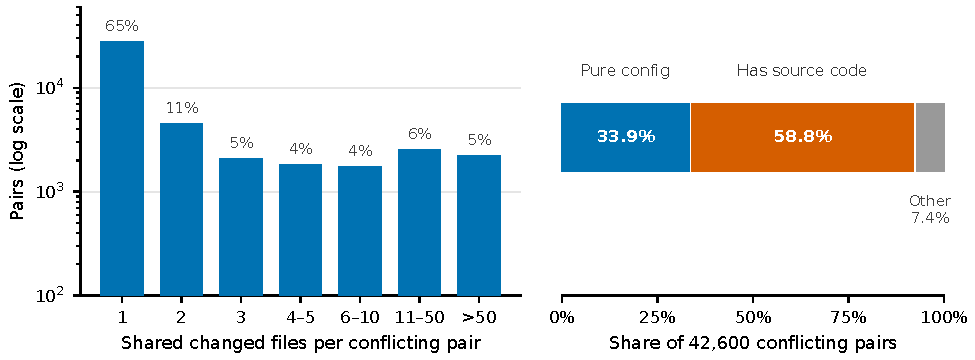
\includegraphics[width=\linewidth]{fig_p1_anatomy.pdf}
\caption{Anatomy of file-overlap ``conflicts'' (42{,}600 pairs). \textbf{Left}: shared files per conflicting pair (log scale): 27{,}709 / 4{,}491 / 2{,}090 / 1{,}821 / 1{,}732 / 2{,}538 / 2{,}219 pairs share 1 / 2 / 3 / 4--5 / 6--10 / 11--50 / $>$50 files. \textbf{Right}: composition: 33.9\% of conflicting pairs share only manifest/lockfile/CI/README files, 58.8\% share at least one source file, 7.4\% share only other docs/misc config.} % src: ev_anatomy.md hist bins; wilson_composition
\label{fig:anatomy}
\end{figure}

\textbf{Most ``conflicts'' are thin and many are noise.}
65.04\% [64.59, 65.50] of conflicting pairs share exactly one file (median 1, mean 10.5, p99 250, max 904). % src: p1_headline_cis.json share_exactly_one_file; verification_log.md anatomy
Classifying shared files with an explicit list (Appendix~\ref{app:filelists}): \textbf{33.88\%} [33.43, 34.33] of conflicting pairs are \emph{pure-config}---every shared file is a manifest, lockfile, CI workflow, Dockerfile, or README---while \textbf{58.76\%} [58.29, 59.23] share at least one genuine source file, and 7.36\% share only other docs/misc config. % src: p1_headline_cis.json pure_config, strict_source; ev_anatomy.md (other 3,135 = 7.36%)
The pure-config share is boundary-sensitive (33.3--35.4\% across reasonable variants; the printed value is exact under the stated lists). % src: verification_log.md anatomy note
The hottest shared basenames are \texttt{README.md} (13{,}803 pair-occurrences) and \texttt{package.json} (9{,}369) (top twelve in Figure~\ref{fig:hotfiles}, Appendix~\ref{app:extrafigs}); % src: verification_log.md anatomy hot files; fig_p1_hotfiles
yet at the occurrence level, config categories are only 9.29\% of shared-file occurrences---config-only conflicts are mostly one-file pairs. % src: ev_anatomy.md §1
So the positive class of the field's conflict label mixes a majority of genuine source collisions with a large minority of mechanical co-edits that plausibly need no verification at all (category B).

\textbf{What file overlap cannot see.}
The duplicate-title pool is the converse error: \textbf{79.55\%} [78.59, 80.49] of near-duplicate-title pairs share \emph{no} file. % src: p1_headline_cis.json dup_no_shared_file
Same-task-twice pairs routinely implement the task in disjoint files (the capgo TS-vs-SQL pairs of \S\ref{sec:intro} are typical). Depth-2 near-misses---no shared file, shared subdirectory---cover 33.1\% of all no-overlap pairs, and cross-agent pairs are near-misses far more often than same-agent ones (45.0\% vs.\ 33.0\% of each group's no-overlap pairs). % src: ev_semantic.md §1 noroot d2 (971/2,160=44.95%; 33.02%)

\textbf{Predictor error anatomy.}
A zero-shot LLM predictor of file overlap from PR text, scored on 5{,}387 held-out pairs enriched to 39.93\% positive, reaches AUC 0.704 and P@100 $=0.96$ \emph{on that enriched 39.9\%-positive test set (random $=0.40$)}. % src: verification_log.md prediction #1,#2,#3
(The predictor is a zero-shot Claude Sonnet, invoked through Claude Code's \texttt{sonnet} alias in headless mode on 2026-08-12 (%% FILL-IN A: exact version string
), prompted, ten pairs per call, with the two PRs' task texts alone (each truncated to 900 characters) to score the probability of a shared changed file; the prompt, scoring harness, enriched test split, and per-pair scores are released as \texttt{test\_pairs\_for\_llm} and \texttt{llm\_scores}.) % src: 04b_llm_t1_claude_code.py; ev_headroom.md
Its confident errors are diagnostic of the label, not the model: all \textbf{7} false positives with predicted probability $\geq$0.9 are duplicate-task sibling pairs implementing the same task in disjoint files---semantically conflicting, textually clean---while the \textbf{468} confident false negatives (21.8\% of positives) are dominated by CHANGELOG/CODEOWNERS/CI-workflow co-edits and mega-PRs---textually colliding, mostly benign (probability distributions by true label in Figure~\ref{fig:llmerr}, Appendix~\ref{app:extrafigs}). % src: verification_log.md prediction #8; design §5.1 error characterization; fig_p1_llmerr
The ground truth the field trains and evaluates against is noisy in precisely the two directions our taxonomy names.

\section{Results II: candidate pools and what lands}
\label{sec:pools}

\textbf{Duplicate work (D).}
The 6{,}945 near-duplicate-title pairs are 1.20\% of all pairs; only 7 are cross-agent---duplication today is overwhelmingly one agent re-issuing its own task. % src: ev_semantic.md pool sizes; cross_agent 7
Outcomes: \textbf{both merged 46.81\%} [45.64, 47.99], exactly one merged 38.66\% [37.52, 39.81], neither 14.53\% [13.72, 15.38]. % src: p1_headline_cis.json dup_*
We emphasize that these are \emph{title-heuristic pool statistics}: agent titles are heavily templated, and similar-titled both-merged pairs can be complementary sub-tasks (stacked or split work) rather than redundant work; the judge-confirmed both-merged-duplicate rate is the first number the released judge run produces, and we do not anticipate it here. %% FILL-IN E: after 06, replace with: ``the judge confirms XX\% [XX, XX] of both-merged duplicate-title pairs as redundant implementations of the same task, implying a landed-redundancy rate of roughly XX\% of the title pool.'' (judge_report.json -> dup_both_merged_D_rate)
 As a pool statistic it is still striking: among the 3{,}251 both-merged pairs the median close gap is \textbf{0.033 hours} (${\sim}2$ minutes) and 94.0\% close within 24 hours (full gap distribution in Figure~\ref{fig:dupgap}, Appendix~\ref{app:extrafigs}). % src: dup_detail.json close_gap_hours; fig_p1_dupgap
That distribution is dominated by one repo (\texttt{mochilang/mochi}, 2{,}469 of 3{,}251); excluding the two mega-repos leaves $n=782$ with median 0.30\,h and 74.9\% within 24\,h---the pattern survives, attenuated. % src: dup_detail.json excl_mega_repos
Verified examples span the spectrum: \texttt{primer/react} \#6356/\#6367 (``Migrate batch of components from Jest to Vitest'', 122 shared files, both merged) and \texttt{mendableai/firecrawl} \#1445/\#1447 (identical titles, both merged) look like landed redundancy; \texttt{appsmithorg/appsmith} \#40674/\#40675 (identical Kanban-widget titles, zero shared files, neither merged) is duplicate effort thrown away. % src: dup_detail.json examples

\textbf{Contradiction (C).}
Explicit contradiction markers are rare: 278 revert-marker pairs (0.05\% of all pairs), of which 35 share a file, 2 are cross-agent, and exactly 1 explicitly cites the partner PR (\texttt{wix/react-native-ui-lib} above); 110 pairs cross-reference the partner's number in either text. % src: verification_log.md revert pool; ev_semantic.md §3
The practical contradiction-candidate signal is \textbf{fix-in-flight}: 7{,}872 file-overlap pairs (18.5\% of conflicting pairs; 2{,}327 distinct later fix-PRs) where the later PR announces a fix while the earlier overlapping PR is still open (a condition implied by co-activity)---roughly $28\times$ the revert pool. % src: ev_semantic.md pool sizes; 7872/278=28.3
Examples: \texttt{567-labs/instructor} \#1553 (add \texttt{api\_key} parameter) $\rightarrow$ \#1554 (``Fix Python 3.9 compatibility issues in \texttt{from\_provider}''); \texttt{514-labs/moose} \#2343 $\rightarrow$ \#2345 (``Fix SSRF vulnerability''). % src: ev_semantic.md §3
Whether the later PR fixes the earlier PR's work or an unrelated bug in the same files is exactly what the judge layer adjudicates.

\textbf{Landed co-edits (H/B).}
30{,}031 pairs (5.2\%) merged both PRs; 6{,}409 of them (21.3\% of both-merged) also share a file, and 47.73\% [46.51, 48.95] of those merged within 24 hours of each other (median gap 27.0\,h). % src: verification_log.md both-merged; p1_headline_cis.json both_merged_shared_gap_lt24h
Whenever the second merge landed on top of the first, someone---agent, maintainer, or rebase bot---performed reconciliation work that no textual conflict rate records.

\section{Results III: outcome coupling}
\label{sec:outcomes}

\begin{figure}[t]
\centering
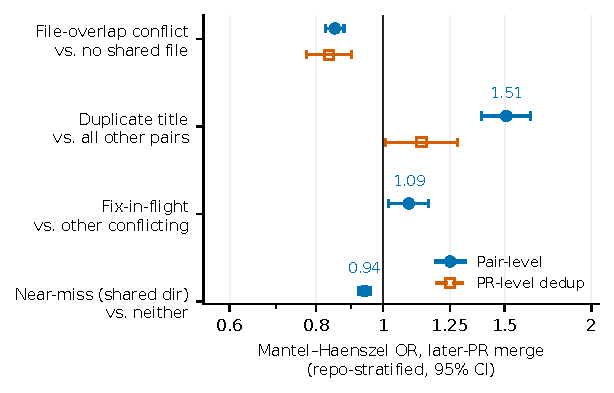
\includegraphics[width=0.62\linewidth]{fig_p1_forest.pdf}
\caption{Repo-stratified Mantel--Haenszel odds ratios (log scale) for the \emph{later} PR's merge odds, with Robins--Breslow--Greenland 95\% CIs. Filled circles: pair-level; open squares: PR-level dedup sensitivity (each distinct later PR counted once). The both-merged pool is excluded: its membership conditions on the outcome.} % src: p1_outcomes.json
\label{fig:forest}
\end{figure}

Merge outcomes come from the corpus merged flags; all associations are observational and none are causal claims. The raw picture: later PRs in file-overlap pairs merge at 73.33\% vs.\ 85.96\% for no-overlap pairs ($-$12.6\,pp; crude OR 0.449 [0.439, 0.459]). % src: p1_outcomes.json a_conflict_vs_none
But conflicts concentrate in burst repos with low per-PR merge rates, so crude ORs confound repo composition with pair-level effects. The defensible estimates are repo-stratified Mantel--Haenszel ORs (Figure~\ref{fig:forest}):

\begin{itemize}
  \item \textbf{File-overlap conflict vs.\ none}: MH OR \textbf{0.851} [0.825, 0.878] over 534 repo strata---within-repo merge odds ${\sim}15\%$ lower, an association far smaller than the crude 0.449 suggests. % src: p1_outcomes.json a_conflict_vs_none
  PR-level dedup sensitivity (each distinct later PR once, $n=24{,}254$): MH 0.836 [0.775, 0.901] (crude 0.588). % src: p1_outcomes.json a_dedup_pr_level
  The estimate is also not driven by near-duplicate pairs: excluding title-Jaccard $\geq 0.5$ pairs gives MH 0.861 [0.834, 0.889]; excluding TF-IDF cosine $\geq 0.7$ pairs gives 0.857 [0.830, 0.884]. % src: mh_robustness.json
  \item \textbf{Duplicate-title vs.\ all other pairs}: crude OR 0.851 [0.799, 0.907] but MH OR \textbf{1.507} [1.390, 1.635] over 207 strata---a Simpson reversal. \emph{Within} a repo, the later PR of a duplicate pair merges \emph{more} often than baseline; the apparent penalty is entirely between-repo composition. One associational reading: duplicates arise from retried, well-scoped tasks that tend to land---which makes the landed-redundancy question sharper, not moot. PR-level dedup: MH 1.137 [1.009, 1.281]. % src: p1_outcomes.json b_dup_title_vs_rest, b_dedup_pr_level
  \item \textbf{Fix-in-flight vs.\ other conflicting pairs}: crude 0.581 [0.552, 0.612], MH \textbf{1.090} [1.019, 1.165] over 334 strata---also reversed: within-repo, later fix-PRs are slightly \emph{more} likely to merge than other conflicting later PRs. % src: p1_outcomes.json c_fif_vs_other_conflict
  \item \textbf{Depth-2 near-miss vs.\ sharing nothing}: MH \textbf{0.940} [0.923, 0.958] over 430 strata (crude 0.610)---a small but statistically significant reduction in within-repo merge odds for pairs invisible to file overlap. % src: p1_outcomes.json d_nearmiss_vs_nothing
  \item \textbf{Both-merged + shared file}: excluded---membership requires the later PR to be merged, so an OR is undefined by construction. % src: p1_outcomes.json e_both_merged_shared_file
\end{itemize}

Two lessons for verification signals. First, the file-overlap association that survives stratification is real but modest (OR 0.85); the dramatic crude gap is repo composition---exactly the confound a verifier trained on pooled data would learn. Second, the two crude-vs-MH sign flips show that na\"ive outcome correlations over this corpus mislead in \emph{direction}, not just magnitude: any pair-level verifier or scheduler evaluated on this data must stratify by repo.

\section{Results IV: when different agents collide---all 99 cases}
\label{sec:crossagent}

Cross-agent pairs are 0.5\% of pairs but share changed files at $3.3\times$ the same-agent rate (24.4\% vs.\ 7.3\%; \S\ref{sec:data}). % src: verification_log.md anatomy
Because the semantic-layer cross-agent evidence is small, we enumerate it exhaustively rather than estimate rates: across the three enumerable pools (both-merged + shared file, duplicate-title, revert) there are exactly \textbf{99} cross-agent pairs\footnote{The companion benchmark paper's T2 suite reports 88 cross-agent pairs because it additionally applies a source-file filter to the both-merged pool; the two counts are consistent.} (90 + 7 + 2; the pools are disjoint). % src: cross_agent_cases.csv; dup_detail.json cross_agent_summary
Table~\ref{tab:crossagent} shows ten exemplars. Per pool: all 90 both-merged-pool pairs merged both PRs \emph{by construction}; of the 7 cross-agent duplicate pairs, none merged both, 2 merged one, 5 merged neither; both revert pairs merged both PRs. (The aggregate 92/99 = 92.9\% both-merged rate is mechanically inflated by the outcome-conditioned pool and should not be quoted alone.) % src: dup_detail.json cross_agent_summary; cross_agent_cases.csv rows
The most frequent unordered agent combinations are Codex+Copilot (27), Codex+Cursor (21), Devin+Cursor (16), and Codex+Claude Code (10); ordered by which agent opened first, Codex$\rightarrow$Cursor (17) and Codex$\rightarrow$Copilot (16) lead. % src: dup_detail.json per_agent_combo (aggregated)
The duplicate cases are the clearest verifier gap: in \texttt{ElectNewt/Distribt}, Codex and Copilot each implemented the outbox pattern for the same microservice within one co-active window---and both PRs died.

\begin{table}[t]
\centering
\caption{Ten of the 99 cross-agent candidate pairs (full table in the artifact). Outcome: M/M = both merged, --/M = later merged only, --/-- = neither.}
\label{tab:crossagent}
\scriptsize
\begin{tabular}{@{}llllrl@{}}
\toprule
Repo & PRs & Agents & Pool & Shared & Outcome \\
\midrule
\texttt{ElectNewt/Distribt} & \#47/\#48 & Codex/Copilot & dup (outbox pattern $\times 2$) & 6 & --/-- \\ % src: cross_agent_cases.csv
\texttt{OpenSprinkler-App} & \#263/\#264 & Copilot/Codex & dup (localStorage fix $\times 2$) & 4 & --/M \\ % src: cross_agent_cases.csv
\texttt{berachain/beacon-kit} & \#2840/\#2841 & Cursor/Codex & dup (balance-proof endpoint $\times 2$) & 6 & --/-- \\ % src: cross_agent_cases.csv
\texttt{liveblocks/liveblocks} & \#2522/\#2523 & Devin/Cursor & dup (same typo fixes) & 3 & --/-- \\ % src: cross_agent_cases.csv
\texttt{airbytehq/airbyte} & \#62941/\#63713 & Claude Code/Devin & revert (base-image rollback) & 0 & M/M \\ % src: cross_agent_cases.csv
\texttt{nodetool-ai/nodetool} & \#158/\#159 & Cursor/Codex & revert (``Revert web changes'') & 0 & M/M \\ % src: cross_agent_cases.csv
\texttt{gofiber/fiber} & \#3508/\#3583 & Codex/Copilot & both-merged & 78 & M/M \\ % src: cross_agent_cases.csv
\texttt{novuhq/novu} & \#8562/\#8584 & Cursor/Devin & both-merged & 248 & M/M \\ % src: cross_agent_cases.csv
\texttt{Significant-Gravitas/AutoGPT} & \#9965/\#10340 & Codex/Claude Code & both-merged & 217 & M/M \\ % src: cross_agent_cases.csv
\texttt{theopenco/llmgateway} & \#208/\#420 & Devin/Cursor & both-merged & 43 & M/M \\ % src: cross_agent_cases.csv
\bottomrule
\end{tabular}
\end{table}

\section{Implications for agent verification}
\label{sec:implications}

Evaluation of coding agents assumes the unit of evaluation is one PR; in deployment the unit that fails is the pair, and this measurement says \emph{what} a valid evaluation target for concurrent agent work has to include. Verifying an agent PR in isolation---the SWE-bench-style contract \citep{swebench,swegym}---misses both failure modes documented here: redundant work that lands twice, often within the hour, and contradictory or interfering work in disjoint files. The verification artifact is the \emph{pair} (and ultimately the co-active set). Concretely: (i) a pair-level verifier should discount the ${\sim}34\%$ of file-overlap alarms that are pure config and attend to the duplicate/near-miss space where 79.6\% of duplicate candidates hide; (ii) Palant\'ir-style horizontal awareness \citep{palantir} and Cassandra-style conflict-aware scheduling \citep{cassandra} have direct agent-fleet analogues, and our pools and forthcoming labels are their evaluation substrate---set-level verification substrates are already emerging, with BulkPR-Bench \citep{bulkprbench} scoring agents on delivering the largest safe subset of a queued PR set, a constructed benchmark our naturally occurring pair labels complement; (iii) any learned verifier must be evaluated repo-stratified, or Simpson reversals will invert its learned associations. Our labels are measurement labels, not yet a benchmark: benchmark hygiene (repo-disjoint splits, gold-only evaluation) is deliberately left to companion work.

\section{Limitations and threats}
\label{sec:limitations}

\begin{figure}[t]
\centering
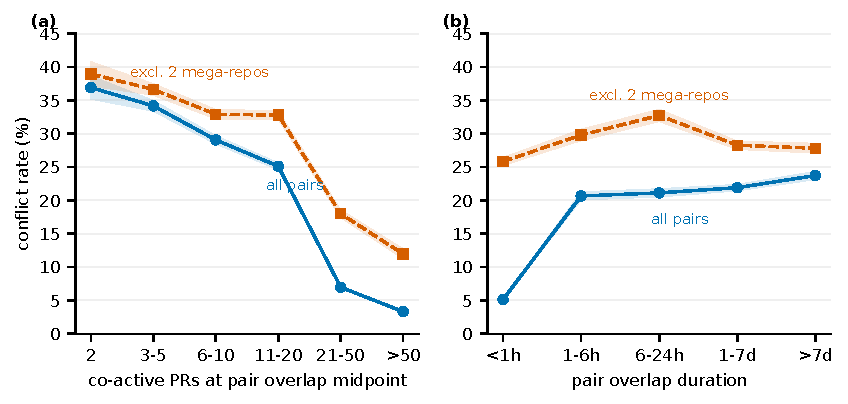
\includegraphics[width=0.8\linewidth]{fig_p1_dose.pdf}
\caption{Apparent dose--response is largely compositional. File-overlap conflict rate vs.\ (a) concurrency at the pair's overlap midpoint and (b) pair overlap duration (left-closed buckets), with Wilson 95\% CI bands; blue circles: all 577{,}045 co-active pairs, vermillion squares: excluding the two mega-repos. Concurrency counts distinct agent PRs whose $[$opened, closed$]$ interval contains the pair's overlap midpoint, incl.\ the pair's own two (minimum 2); never-closed PRs carry a censored global-max close time, inflating high-concurrency counts. All-pairs rates fall from 36.90\% ($n=2{,}957$) at concurrency 2 to 3.32\% ($n=302{,}602$) above 50, vs.\ a far shallower 38.93\% to 11.97\% excluding mega-repos; in (b) the all-pairs rate rises from 5.13\% ($n=499{,}538$) under 1\,h to 23.72\% ($n=17{,}808$) beyond 7\,d, yet stays within 25.82--32.72\% excluding mega-repos.} % src: fig_p1_dose crosscheck (all bucket rates and n's match); verification_log.md anatomy dose-response
\label{fig:dose}
\end{figure}

\textbf{Pools are heuristics.} All five pools are recall-oriented candidate sets; none is a confirmed semantic-conflict label. Title heuristics miss same-task-different-title duplicates (the predictor's 7 false positives prove such pairs exist outside the pool) and admit templated-title false positives; because pool sizes bound prevalence from below only under perfect precision, which we do not claim, we treat them as recall-oriented candidate volumes and defer all prevalence claims to the judged layer (\S\ref{sec:pipeline}). The 46.8\% both-merged duplicate rate in particular is a pool statistic pending judge confirmation.
\textbf{Truncated text.} Text pools were grepped over bodies truncated at 1{,}200 characters (21.58\% at the cap); title-based pools (D, revert) are unaffected because titles are not truncated; the fix-in-flight and cross-reference counts, which read bodies, are lower bounds under truncation and will be recomputed over untruncated bodies for the camera-ready. % src: verification_log.md prediction #10
\textbf{Corpus concentration.} Two repos hold 87.3\% of pairs and 92.2\% of pairs are Codex--Codex (concentration curves in Figure~\ref{fig:concentration}, Appendix~\ref{app:extrafigs}); we mitigate with MH stratification, per-repo caps, and mega-repo-excluded sensitivity numbers (reported wherever a headline depends on them), but the population is one platform fanning out work far more than agents of different vendors competing. The duration dose-response reported by \citet{xu2026agentprs} is compositional in this data (flat once mega-repos are excluded), and the concurrency gradient likewise attenuates (Figure~\ref{fig:dose}). % src: verification_log.md anatomy dose-response; fig_p1_dose; fig_p1_concentration
\textbf{Outcome proxies and confounding.} Merged flags are trustworthy but close timestamps only proxy merge times; MH ORs are associations---task difficulty, PR size, and maintainer behavior are unmodeled confounders, and no causal claim is made.
\textbf{Category I} is presented as a candidate signal only: depth-2 co-location neither implies nor is implied by real dependency interference, and its validation requires the repo-browsing deep-dive specified in \S\ref{sec:pipeline}.
\textbf{Definitional sensitivity.} Pure-config share moves 33.3--35.4\% across reasonable file-class boundaries and fix-in-flight moves 7{,}791--8{,}281 across keyword rules; we print exact values under stated definitions and release the classifiers. % src: verification_log.md anatomy note; verification_log.md fix-in-flight rule-range

\paragraph{Ethics and licensing.}
This study analyzes public GitHub PR metadata (titles, bodies, file paths, merge status) of agent-authored PRs via the AIDev dataset \citep{li2026aidev}, used under its published license and terms; we redistribute no repository source code. The data concerns automated agents' contributions to public repositories; the only human-identifying information is public GitHub metadata, which we do not augment, and repository/PR identifiers appear here exactly as publicly visible. Measurement of agent duplication and interference could inform both better coordination and adversarial gaming of merge queues; we judge the transparency benefit to maintainers---who currently absorb reconciliation costs invisibly---to outweigh that risk.

\paragraph{Reproducibility.}
All pool definitions are stated exactly (\S\ref{sec:pooldefs}, Appendix~\ref{app:filelists}); every reported number derives from the released derivation scripts over AIDev-pop or from cited prior work. Proportion CIs are Wilson 95\% intervals at the stated numerators/denominators; MH ORs use $\sum(a_i d_i/N_i)/\sum(b_i c_i/N_i)$ over repo strata (strata lacking either exposure arm contribute nothing; informative strata counts reported per contrast) with Robins--Breslow--Greenland CIs on the log scale. The pair table, pool membership flags, judging frame with inclusion probabilities, calibration sheet, judge and scoring scripts, cross-agent case table, and figure-generation code are released with the submission; judged labels follow.

\section{Conclusion}

File overlap is the verification signal the agent-concurrency literature measures and orchestrators act on. On 577{,}045 co-active agent PR pairs it is wrong in both directions: a third of its positives are config-only noise, while four-fifths of duplicate-work candidates---nearly half of which land both PRs, often within the hour---are invisible to it, and within-repo outcome analysis reverses the sign of two of its crude associations. We provide the taxonomy, the exact candidate pools, the outcome coupling, the exhaustive cross-agent case study, and a pre-registered judge-and-validate pipeline whose population-weighted prevalence estimates will complete the picture. Verifying agents means verifying their concurrent work as pairs---and the field's current pair-level signal is not up to the job.

\bibliographystyle{plainnat}
\bibliography{references}

\appendix

\section{File-classification lists}
\label{app:filelists}

\sloppy
The config/source classification of \S\ref{sec:anatomy} uses these exact lists (case-insensitive basename/path matching). % src: verification_log.md file-class lists
\textbf{Lockfiles}: \texttt{*.lock}, \texttt{pnpm-lock.yaml}, \texttt{bun.lockb}, \texttt{package-lock.json}.
\textbf{Manifests}: \texttt{package.json}, \texttt{pom.xml}, \texttt{Cargo.toml}, \texttt{Gemfile}, \texttt{composer.json}, \texttt{build.gradle}, \texttt{setup.py}, \texttt{setup.cfg}, \texttt{go.mod}, \texttt{go.sum}, \texttt{requirements*}, \texttt{pyproject.toml}.
\textbf{Infra}: \texttt{Dockerfile*}, \texttt{docker-compose*}, \texttt{.github/workflows/*}.
\textbf{README}: \texttt{README*}.
A pair is \emph{pure-config} if every shared file falls in the above sets. A pair is \emph{strict-source} if at least one shared file is outside the above sets and also outside \textbf{docs} (\texttt{.md}, \texttt{.rst}, \texttt{.txt}, \texttt{CHANGELOG*}) and \textbf{misc config} (\texttt{.gitignore}, \texttt{.env*}, and other \texttt{.yaml}, \texttt{.yml}, \texttt{.json}, \texttt{.toml}, \texttt{.ini}, \texttt{.cfg} files). Remaining pairs (7.36\%) share only docs/misc-config files. % src: ev_anatomy.md (other 3,135/42,600)

\section{Additional figures}
\label{app:extrafigs}

Figures~\ref{fig:llmerr}--\ref{fig:dupgap} supplement the main-text analyses: the predictor error anatomy of \S\ref{sec:anatomy}, the hottest shared basenames behind the file-class composition of \S\ref{sec:anatomy}, the repository concentration underlying every mega-repo-excluded sensitivity number (\S\ref{sec:limitations}), and the close-gap distribution behind the landed-redundancy statistic of \S\ref{sec:pools}.

\begin{figure}[ht]
\centering
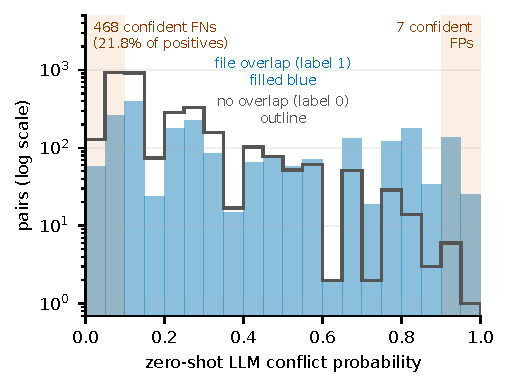
\includegraphics[width=0.7\linewidth]{fig_p1_llmerr.pdf}
\caption{Predictor error anatomy: histograms (bin width 0.05, log-scale $y$) of the zero-shot LLM conflict probability on the frozen test set ($n=5{,}387$ pairs; 2{,}151 positives, 39.93\%), split by true file-overlap label. 468 label-1 pairs (21.8\% of positives) receive probability $\leq0.1$ (confident false negatives) while only 7 label-0 pairs receive probability $\geq0.9$ (confident false positives); both thresholds are inclusive. The zero-shot AUC of 0.7044 on this set comes from the audited leaderboard, not recomputed here.} % src: fig_p1_llmerr crosscheck (468/7/5,387/39.93% match)
\label{fig:llmerr}
\end{figure}

\begin{figure}[ht]
\centering
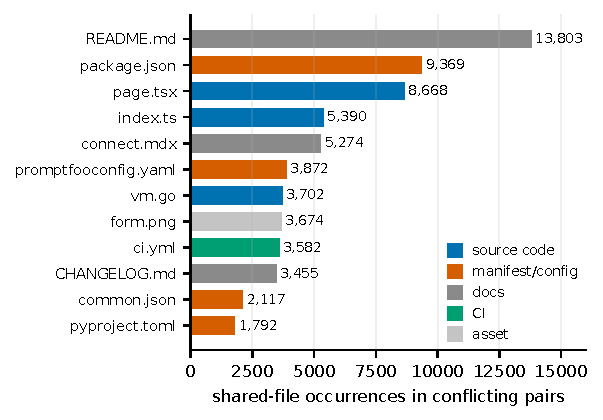
\includegraphics[width=0.78\linewidth]{fig_p1_hotfiles.pdf}
\caption{The twelve most frequent basenames across the shared-file sets of the 42{,}600 file-overlap conflicting pairs, colored by file class. Counts are pair$\times$shared-file occurrences: each file in a conflicting pair's shared set contributes its basename once per pair (two same-named files in one pair's shared set count twice). \texttt{README.md} 13{,}803 (docs), \texttt{package.json} 9{,}369 (manifest/config), \texttt{page.tsx} 8{,}668 (source), \texttt{index.ts} 5{,}390 (source), \texttt{connect.mdx} 5{,}274 (docs), \texttt{promptfooconfig.yaml} 3{,}872 (manifest/config), \texttt{vm.go} 3{,}702 (source), \texttt{form.png} 3{,}674 (asset), \texttt{ci.yml} 3{,}582 (CI), \texttt{CHANGELOG.md} 3{,}455 (docs), \texttt{common.json} 2{,}117 (manifest/config), \texttt{pyproject.toml} 1{,}792 (manifest/config). Classes are hand-assigned per basename (\texttt{common.json}, a locale/config file, is classed manifest/config; \texttt{connect.mdx} as docs).} % src: fig_p1_hotfiles crosscheck (all 12 counts match)
\label{fig:hotfiles}
\end{figure}

\begin{figure}[ht]
\centering
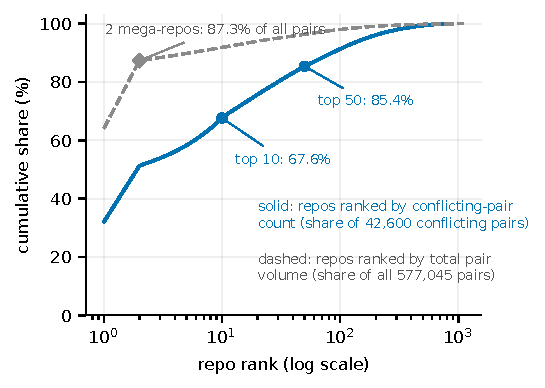
\includegraphics[width=0.7\linewidth]{fig_p1_concentration.pdf}
\caption{Repository concentration ($x$: repo rank, log scale; $y$: cumulative share; 1{,}100 repos on each curve). The two curves use \emph{different} rankings, as labeled on the figure. Blue solid: repos ranked by conflicting-pair count, cumulative share of the 42{,}600 conflicting pairs---the top 10 repos hold 67.6\% and the top 50 hold 85.4\%. Gray dashed: repos ranked by total pair volume, cumulative share of all 577{,}045 pairs---the two mega-repos (\texttt{mochilang/mochi}, 369{,}597 pairs; \texttt{MontrealAI/AGI-Alpha-Agent-v0}, 134{,}132) are the top two and hold 87.3\%.} % src: fig_p1_concentration crosscheck (67.6/85.4/87.3 and repo counts match)
\label{fig:concentration}
\end{figure}

\begin{figure}[ht]
\centering
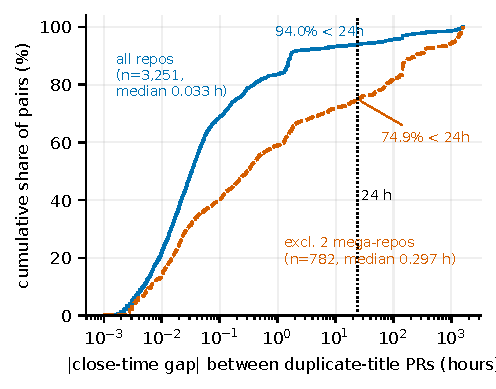
\includegraphics[width=0.7\linewidth]{fig_p1_dupgap.pdf}
\caption{ECDF of the absolute close-time gap in hours (log $x$-axis) between the two PRs of both-merged duplicate-title pairs; close time proxies merge time. All repos: $n=3{,}251$, median 0.033\,h, 94.0\% within 24\,h. Excluding the two mega-repos: $n=782$, median 0.297\,h, 74.9\% within 24\,h. Underlying pool: 6{,}945 duplicate-title pairs (normalized-title match: token-set Jaccard $\geq0.5$ or $\geq$15-character containment, both titles $\geq$3 tokens); the both-merged subset is shown. Zero gaps (simultaneous closes) are drawn at 0.001\,h purely for the log axis; medians are unaffected.} % src: fig_p1_dupgap crosscheck (3,251/0.033/94.0; 782/0.297/74.9 match)
\label{fig:dupgap}
\end{figure}

\end{document}
